%----------------------------------------------------------------------------------------
%	PACKAGES AND OTHER DOCUMENT CONFIGURATIONS
%----------------------------------------------------------------------------------------

\documentclass[fleqn,10pt]{SelfArx} % Document font size and equations flushed left

\usepackage[english]{babel}

\usepackage{lipsum}

\usepackage{graphicx}

\usepackage{appendix}

\usepackage{amsmath}

%----------------------------------------------------------------------------------------
%	COLUMNS
%----------------------------------------------------------------------------------------

\setlength{\columnsep}{0.55cm} % Distance between the two columns of text
\setlength{\fboxrule}{0.75pt} % Width of the border around the abstract

%----------------------------------------------------------------------------------------
%	COLORS
%----------------------------------------------------------------------------------------

\definecolor{color1}{RGB}{0,0,90} % Color of the article title and sections
\definecolor{color2}{RGB}{0,20,20} % Color of the boxes behind the abstract and headings

%----------------------------------------------------------------------------------------
%	HYPERLINKS
%----------------------------------------------------------------------------------------

\usepackage{hyperref}

\hypersetup{
	hidelinks,
	colorlinks,
	breaklinks=true,
	urlcolor=color2,
	citecolor=color1,
	linkcolor=color1,
	bookmarksopen=false,
	pdftitle={Title},
	pdfauthor={Author},
}

%----------------------------------------------------------------------------------------
%	ARTICLE INFORMATION
%----------------------------------------------------------------------------------------

\JournalInfo{ENGN3712: Major Research Project}
\Archive{Mid Project Report}

\PaperTitle{Bringing Extract Method Refactoring to the Rust Programming Language:
Experiments with REM}

\Authors{Matthew Britton\textsuperscript{1}, Supervisor: Alex Potanin\textsuperscript{2}}
\affiliation{\textsuperscript{1}\textit{School of Engineering, The Australian
National University. | matt.britton@anu.edu.au}}
\affiliation{\textsuperscript{2}\textit{School of Computing, The Australian
National University. | alex.potanin@anu.edu.au}}

\Keywords{Rust}
\newcommand{\keywordname}{Keywords}

%----------------------------------------------------------------------------------------
%	ABSTRACT
%----------------------------------------------------------------------------------------

\Abstract{Lorem ipsum dolor sit amet, consectetur adipiscing elit. Sed auctor, nunc nec}

%----------------------------------------------------------------------------------------

\begin{document}

\maketitle

\tableofcontents

\listoffigures

\listoftables


%----------------------------------------------------------------------------------------
%	ARTICLE CONTENTS
%----------------------------------------------------------------------------------------

\section{Introduction}

\section{Theoretical Background}



\section{Literature Review}

\section{Experimental Methods}

\section{Results and Discussion}

\section{Future Work}

\section{Conclusions}


%------------------------------------------------

\phantomsection
\section*{Acknowledgments}

I would like to thank my supervisor, Alex Potanin, for his guidance and support.
Additionally, I would like to thank Sasha Pak for listening in on all of our
meetings and providing valuable feedback. Finally, I would like to thank Sewen
Thy, the original developer of REM, for his help in understanding the project
and his assistance in getting me started.
\addcontentsline{toc}{section}{Acknowledgments}

So long and thanks for all the fish \cite{Figueredo:2009dg, Smith:2012qr}.

%----------------------------------------------------------------------------------------
%	REFERENCE LIST
%----------------------------------------------------------------------------------------

\phantomsection
\bibliographystyle{unsrt}
\bibliography{ref.bib}

\renewcommand{\thesection}{A\arabic{section}}
\onecolumn
\section*{Appendices}
\addcontentsline{toc}{section}{Appendices}

\setcounter{section}{0}

\section{Appendix 1}


\section{Appendix 2}

\section{Lifetime Repair \cite{AdventureOfALifetime}}
\label{app:lifetime_repair}

% \begin{algorithm}
%     \caption{FixLifetimes}
%     \textbf{Input}: a cargo manifest file CARGO\_MANIFEST for the whole project, extracted function EF \\
%     \textbf{Output}: patched extracted function EF'
%     \begin{algorithmic}[1]
%         \State $EF' \gets$ clone EF
%         \State $EF' \gets$ update EF' by annotating each borrow in EF'.params and EF'.ret with a fresh lifetime where none exists
%         \State $EF' \gets$ update EF' by adding the freshly introduced lifetimes to the list of lifetime parameters in EF'.sig
%         \Loop
%             \State $err \gets$ (cargo check CARGO\_MANIFEST).errors
%             \If{$err = \emptyset$}
%                 \State break
%             \EndIf
%             \State $suggestions \gets$ collect lifetime bounds suggestions from err
%             \If{$suggestions = \emptyset$}
%                 \State raise RefactorError
%             \EndIf
%             \State $EF' \gets$ apply suggestions to EF'
%         \EndLoop
%         \State collapse the cycles in the where clause of EF'.sig
%         \State apply elision rules
%     \end{algorithmic}
% \end{algorithm}

\begin{figure*}[h!]
    \centering
    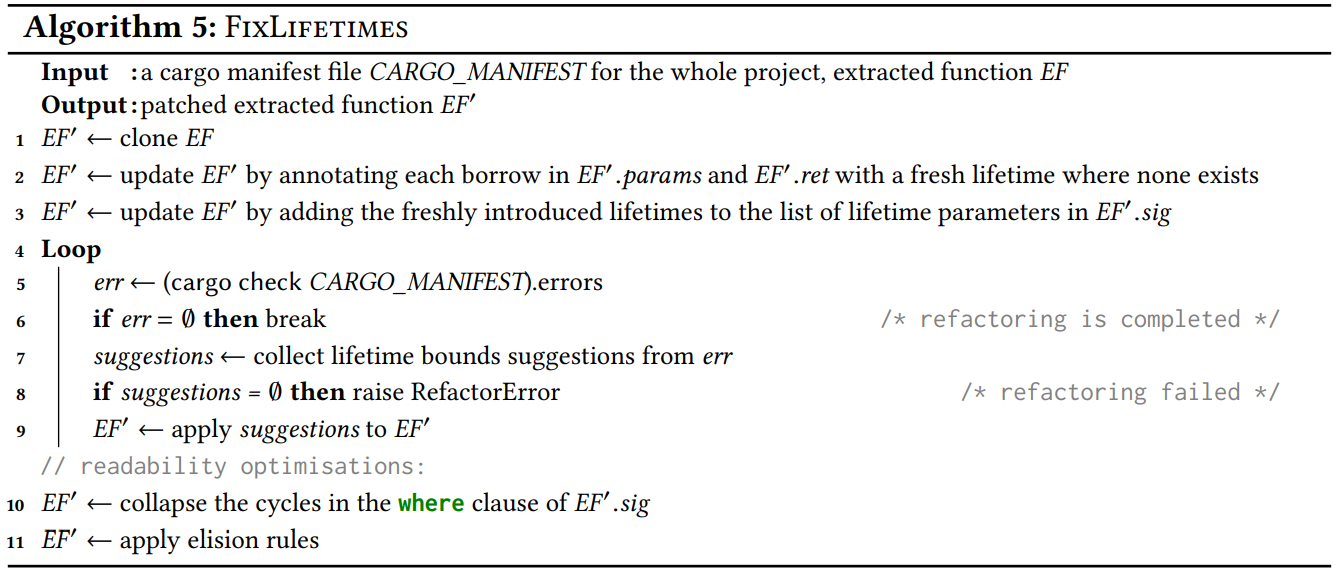
\includegraphics[width=\textwidth]{figures/algo_5.png}
    % \caption{Lifetime Repair}
    \label{fig:algo_5}
\end{figure*}

%----------------------------------------------------------------------------------------

\end{document}